\begin{frame}
	\myheading{Module 3.4: Learning Parameters : Gradient Descent}
\end{frame}
\begin{frame}
	\begin{columns}
		\column{0.4\textwidth}
		\begin{overlayarea}{\textwidth}{\textheight}
			\only<1-2>{
				\begin{center}
					\begin{tikzpicture}
	\node (input0) at (8,-0.1)  {$x_{1}$};
	\node (input1) at (9,-0.1)  {$x_{2}$};
	\node (input2) at (10,-0.1)  {$..$};
	\node (input3) at (11,-0.1)  {$..$};
	\node (input4) at (12,-0.1)  {$x_{n}$};
	\node (input5) at (7,-0.1)  {$x_{0}=1$};

	\node [hidden_neuron] (neuron1) at (10,2)  {};


	\node (output0)  at (10,3.5) {$y$};

	\draw [->] (input0) -- (neuron1);
	\draw [->] (input1) -- (neuron1);
	\draw [->] (input2) -- (neuron1);
	\draw [->] (input3) -- (neuron1);
	\draw [->] (input4) -- (neuron1);
	\draw [->] (input5) -- (neuron1);

	\draw [->] (neuron1) -- (output0);

	\node (formula)[scale=.8] at (8.4,0.6) {$w_{1}$};
	\node (formula)[scale=.8] at (9.1,0.6) {$w_{2}$};
	\node (formula)[scale=.8] at (9.8,0.6) {$..$};
	\node (formula)[scale=.8] at (10.4,0.6) {$..$};
	\node (formula)[scale=.8] at (11.1,0.6) {$w_{n}$};
	\node (formula)[scale=.8] at (7.2,0.6) {$w_{0} = -\theta$};

\end{tikzpicture}

				\end{center}
			}
			\only<3->{
				\begin{center}
					\begin{tikzpicture}
	\node [neuron] (neuron0) at (1,6)  {$\sigma$} ;
	\node (input1) at (-1,6)  {$x$};
	\node (input0) at (-1,5)  {$1$};

	\onslide<4->{\node (w) at (-0.25,5.8)  {$w$};}
	\onslide<4->{\node (b) at (-0.25,5.2)  {$b$};}

	\node (output0) at (3,6)  {$\hat{y} = f(x)$};
	\onslide<4->{\node (formula) at (0,4) {$f(x)= \frac{1}{1+e^{-(w\cdot x + b)}}$};}
	\draw [->] (input0) -- (neuron0);
	\draw [->] (input1) -- (neuron0);
	\draw [->] (neuron0) -- (output0);
\end{tikzpicture}
				\end{center}
			}
		\end{overlayarea}
		\column{0.6\textwidth}
		\begin{overlayarea}{\textwidth}{\textheight}
			\begin{itemize}\justifying
				\item<1-> With this setup in mind, we will now focus on this \textbf{model} and discuss an \textbf{algorithm} for learning the \textbf{parameters} of this model from some given \textbf{data}
				\item<2-> $\sigma$ stands for the sigmoid function (logistic function in this case)
				\item<3-> For ease of explanation, we will consider a very simplified version of the model having just 1 input
				\item<4-> Further to be consistent with the literature, from now on we will refer to $w_0$ as $b$ (bias)
				\item<5-> Lastly, instead of considering the problem of predicting like/dislike we will assume that we want to predict $criticsRating (y)$ given  $imdbRating (x)$ (for no particular reason)
			\end{itemize}
		\end{overlayarea}
	\end{columns}
\end{frame}


\begin{frame}
	\begin{columns}
		\column{0.5\textwidth}
		\begin{overlayarea}{\textwidth}{\textheight}
			\begin{center}
				\begin{tikzpicture}
	\node [neuron] (neuron0) at (1,6)  {$\sigma$} ;
	\node (input1) at (-1,6)  {$x$};
	\node (input0) at (-1,5)  {$1$};

	\onslide<4->{\node (w) at (-0.25,5.8)  {$w$};}
	\onslide<4->{\node (b) at (-0.25,5.2)  {$b$};}

	\node (output0) at (3,6)  {$\hat{y} = f(x)$};
	\onslide<4->{\node (formula) at (0,4) {$f(x)= \frac{1}{1+e^{-(w\cdot x + b)}}$};}
	\draw [->] (input0) -- (neuron0);
	\draw [->] (input1) -- (neuron0);
	\draw [->] (neuron0) -- (output0);
\end{tikzpicture}
			\end{center}
			\only<5->{
				\vspace{-0.2in}
				\begin{figure}[!htp]
					\begin{center}
						\includegraphics<5-8>[scale=0.3]{images/module4/2sample_points.png}
						\includegraphics<9->[scale=0.3]{images/module4/2sample_points_sigmoid.png}
					\end{center}
				\end{figure}
			}
		\end{overlayarea}
		\column{0.5\textwidth}<2->
		\begin{overlayarea}{\textwidth}{\textheight}
			\only<2-4>{
				\begin{block}<2-4>{Input for training}
					$\{x_i, y_i\}^{N}_{i=1} \rightarrow N$ pairs of $(x,y)$
				\end{block}
				\begin{block}<3-4>{Training objective}
					Find $w$ and $b$ such that:\\
					$\displaystyle{\minimize_{w,b} \mathscr{L}(w,b) = \sum_{i=1}^{N} (y_i - f(x_i))^2}$
				\end{block}
			}
			\only<5->{
				\begin{block}{What does it mean to train the network?}
					\begin{itemize}\justifying
						\item<5-> Suppose we train the network with $ (x, y) = (0.5, 0.2)$ and $(2.5, 0.9)$
						\item<6-> At the end of training we expect to find w*, b* such that:
						\item<7-> $f(0.5) \rightarrow 0.2$ and  $f(2.5) \rightarrow 0.9$
					\end{itemize}
				\end{block}
				\begin{block}<8->{In other words...}
					\begin{itemize}\justifying
						\item We hope to find a sigmoid function such that $(0.5, 0.2)$ and $(2.5, 0.9)$ lie on this sigmoid
					\end{itemize}
				\end{block}
			}
		\end{overlayarea}
	\end{columns}
\end{frame}

%\subsection{Curve-fitting}
\begin{frame}
	\fontsize{16pt}{7.2}\selectfont
	\textit{Let us see this in more detail....}
\end{frame}

\begin{frame}
	\begin{columns}
		\column{0.35\textwidth}
		\begin{overlayarea}{\textwidth}{\textheight}
			\begin{onlyenv}<1->
				\begin{figure}[!htp]
					\begin{center}
						\includegraphics<1-2>[scale=0.3]{images/module4/2sample_points.png}
						\includegraphics<3-11>[scale=0.3]{images/module4/random/sig0.png}
						\includegraphics<12>[scale=0.3]{images/module4/random/sig1.png}
						\includegraphics<13>[scale=0.3]{images/module4/random/sig2.png}
						\includegraphics<14>[scale=0.3]{images/module4/random/sig3.png}
						\includegraphics<15>[scale=0.3]{images/module4/random/sig4.png}
						\includegraphics<16->[scale=0.3]{images/module4/random/sig5.png}
					\end{center}
				\end{figure}
			\end{onlyenv}
		\end{overlayarea}
		\column{0.65\textwidth}
		\begin{overlayarea}{\textwidth}{\textheight}
			\only<2-5>{
				\begin{itemize}\justifying
					\item Can we try to find such a $w*, b*$ manually
					\item<3-> Let us try a random guess.. (say, $w=0.5, b=0$)
					\item<4-> Clearly not good, but how bad is it ?
					\item<5-> Let us revisit $\mathscr{L}(w,b)$ to see how bad it is ...
				\end{itemize}
			}
			\only<6-10>{
				\begin{align*}
					\onslide<6->{\mathscr{L}(w,b) & = \frac{1}{2} * \sum_{i=1}^{N} (y_i - f(x_i))^2}     \\
					\onslide<7->{                 & = \frac{1}{2} * (y_1 - f(x_1))^2 + (y_2 - f(x_2))^2} \\
					\onslide<8->{                 & = \frac{1}{2} * (0.9 - f(2.5))^2 + (0.2 - f(0.5))^2} \\
					\onslide<9->{                 & = 0.073}
				\end{align*}
				\only<10->{\parbox[c][50pt][c]{230pt}{We want $\mathscr{L}(w,b)$ to be as close to 0 as possible}}
			}
			\only<11-> {
				Let us try some other values of w, b
				\begin{flushleft}
					\begin{table}
						\begin{tabular}{ccc}
							\hline
							\hline
							$w$               & $b$   & $\mathscr{L}(w,b)$ \\
							\hline
							\hline
							0.50              & 0.00  & 0.0730             \\
							\only<12-> {-0.10 & 0.00  & 0.1481}            \\
							\only<13-> {0.94  & -0.94 & 0.0214}            \\
							\only<14-> {1.42  & -1.73 & 0.0028}            \\
							\only<15-> {1.65  & -2.08 & 0.0003}            \\
							\only<16-> {1.78  & -2.27 & 0.0000}            \\
							\hline
							\hline
						\end{tabular}
					\end{table}
				\end{flushleft}
				\only<12>{\parbox[c][50pt][c]{230pt}{Oops!! this made things even worse...}}
				\only<13>{\parbox[c][50pt][c]{230pt}{Perhaps it would help to push w and b in the other direction...}}
				\only<14-15>{\parbox[c][50pt][c]{230pt}{Let us keep going in this direction, \textit{i.e.}, increase $w$ and decrease $b$}}
				\only<16>{\parbox[c][50pt][c]{230pt}{With some guess work and intuition we were able to find the right values for $w$ and $b$}}
			}
		\end{overlayarea}
	\end{columns}
\end{frame}

%\subsection{Error surfaces}
\begin{frame}
	\fontsize{16pt}{7.2}\selectfont
	\textit{Let us look at something better than our ``guess work'' algorithm....}
\end{frame}

\begin{frame}
	\begin{columns}
		\column{0.5\textwidth}
		\begin{overlayarea}{\textwidth}{\textheight}
			\begin{onlyenv}<1->
				\begin{figure}[!htp]
					\begin{center}
						\includegraphics<2->[scale=0.5]{images/module4/error_surface1.png}
					\end{center}
				\end{figure}
			\end{onlyenv}
		\end{overlayarea}

		\column{0.5\textwidth}
		\begin{overlayarea}{\textwidth}{\textheight}
			\begin{itemize}\justifying
				\item Since we have only 2 points and 2 parameters ($w$, $b$) we can easily plot $\mathscr{L}(w,b)$ for different values of ($w$, $b$) and pick the one where $\mathscr{L}(w,b)$ is minimum
				\item<3-> But of course this becomes intractable once you have many more data points and many more parameters !!
				\item<4-> Further, even here we have plotted the error surface only for a small range of ($w$, $b$) [from $(-6, 6)$ and not from $(-\inf, \inf)$]
			\end{itemize}
		\end{overlayarea}
	\end{columns}
\end{frame}

\begin{frame}
	\fontsize{16pt}{7.2}\selectfont
	\textit{Let us look at the geometric interpretation of our ``guess work'' algorithm in terms of this error surface}
\end{frame}

\begin{frame}
	\begin{columns}
		\column{0.5\textwidth}
		\begin{overlayarea}{\textwidth}{\textheight}
			\begin{onlyenv}<1->
				\begin{figure}[!htp]
					\begin{center}
						\includegraphics<1>[scale=0.4]{images/module4/2sample_points.png}
						\includegraphics<2>[scale=0.4]{images/module4/random/sig0.png}
						\includegraphics<3>[scale=0.4]{images/module4/random/sig1.png}
						\includegraphics<4>[scale=0.4]{images/module4/random/sig2.png}
						\includegraphics<5>[scale=0.4]{images/module4/random/sig3.png}
						\includegraphics<6>[scale=0.4]{images/module4/random/sig4.png}
						\includegraphics<7->[scale=0.4]{images/module4/random/sig5.png}
					\end{center}
				\end{figure}
			\end{onlyenv}
		\end{overlayarea}
		\column{0.5\textwidth}
		\begin{overlayarea}{\textwidth}{\textheight}
			\begin{onlyenv}<1->
				\begin{figure}[!htp]
					\begin{center}
						\includegraphics<1>[scale=0.5]{images/module4/error_surface1.png}
						\includegraphics<2>[scale=0.5]{images/module4/random/error0.png}
						\includegraphics<3>[scale=0.5]{images/module4/random/error1.png}
						\includegraphics<4>[scale=0.5]{images/module4/random/error2.png}
						\includegraphics<5>[scale=0.5]{images/module4/random/error3.png}
						\includegraphics<6>[scale=0.5]{images/module4/random/error4.png}
						\includegraphics<7->[scale=0.5]{images/module4/random/error5.png}
					\end{center}
				\end{figure}
			\end{onlyenv}
		\end{overlayarea}
	\end{columns}
\end{frame}


\begin{frame}
	\fontsize{16pt}{7.2}\selectfont
	\textit{Now let us see if there is a more efficient and principled way of doing this}
\end{frame}

\begin{frame}
	\begin{block}{Goal}
		Find a better way of traversing the error surface so that we can reach the minimum value quickly without resorting to brute force search!
	\end{block}
\end{frame}


\begin{frame}
	\begin{overlayarea}{\textwidth}{\textheight}
		\begin{tikzpicture}[inner sep=2mm]
	\node (theta) at (1,6)  {\only<1->{$\theta = [w, b]$}} ;
	\node (deltatheta) at (1,5)  {\only<2->{$\Delta\theta = [\Delta w, \Delta b]$}} ;
	\node (thetanew) at (1,3)  {\only<9->{$\theta_{new} = \theta + \eta\cdot\Delta\theta$}} ;
	\node (text1) at (-1,7)  {\only<1->{{\parbox[c][20pt][c]{110pt}{vector of parameters, say, randomly initialized}}}};
	\node (text2) at (-2,4)  {\only<2->{{\parbox[c][20pt][c]{70pt}{change in the values of w, b}}}};
	\node (text3) at (6,2)  {\only<10->{{\parbox[c][20pt][c]{190pt}{\textbf{Question:} What is the right $\Delta\theta$ to use ?}}}};

	\node (text4) at (9,6)  {\only<5->{{\parbox[c][40pt][c]{120pt}{We moved in the direction of $\Delta\theta$}}}};

	\node (text5) at (9,4)  {\only<6->{{\parbox[c][60pt][c]{120pt}{Let us be a bit conservative: move only by a small amount $\eta$}}}};

	\node (text4) at (6,1)  {\only<11->{{\parbox[c][20pt][c]{190pt}{The answer comes from Taylor series}}}};


	\only<1->{\draw [->] (text1) to [out=-90,in=180] (theta)};
	\only<2->{\draw [->] (text2) to [out=90,in=180] (deltatheta)};
	\only<10->{\draw [->] (text3) to [out=90,in=0] (thetanew)};

	\only<3->{\draw [->] (3,5) to node[left]{$\theta$} (4,7)};
	\only<3->{\draw [->] (3,5) to node[below]{$\Delta\theta$} (6,5)};
	\only<4->{\draw [dashed] (4,7) to (7,7)};
	\only<4->{\draw [dashed] (6,5) to (7,7)};
	\only<4->{\draw [->] (3,5) to node[left]{$\theta_{new}$} (7,7)};

	\begin{scope}[color=red]
		\only<7->{\draw [->] (3,5) to node[below]{$\eta\cdot\Delta\theta$} (4,5)};
		\only<8->{\draw [dashed] (4,7) to (5,7)};
		\only<8->{\draw [dashed] (4,5) to (5,7)};
		\only<8->{\draw [->] (3,5) to  (5,7)};
	\end{scope}
\end{tikzpicture}
	\end{overlayarea}

\end{frame}

%\subsection{Taylor series}
\begin{frame}
	\begin{overlayarea}{\textwidth}{\textheight}
		For ease of notation, let $\Delta\theta = u$, then from Taylor series, we have,
		\begin{align*}
			\only<2->{\mathscr{L}(\theta + \eta u) & =  \mathscr{L}(\theta)+ \eta*u^T \nabla\mathscr{L}(\theta) + \frac{\eta^2}{2!}*u^T \nabla^2\mathscr{L}(\theta)u + \frac{\eta^3}{3!}*... + \frac{\eta^4}{4!}*...} \\
			\only<3->{                             & = \mathscr{L}(\theta)+ \eta*u^T \nabla\mathscr{L}(\theta) \text{  } [\textit{$\eta$ is typically small, so $\eta^2, \eta^3,.. \rightarrow 0$}]}
		\end{align*}
		\only<4->{Note that the move ($\eta u$) would be favorable only if,}
		\begin{align*}
			\only<4->{ & \mathscr{L}(\theta + \eta u) - \mathscr{L}(\theta) < 0 [\textit{i.e., if the new loss is less than the previous loss}]} \\
			\only<5->{\intertext {This implies,}}
			\only<5->{ & u^T \nabla\mathscr{L}(\theta) < 0}
		\end{align*}
	\end{overlayarea}
\end{frame}

\begin{frame}
	\begin{overlayarea}{\textwidth}{\textheight}
		Okay, so we have,
		\begin{align*}
			u^T \nabla\mathscr{L}(\theta) < 0
		\end{align*}
		\only<1->{But, what is the range of $u^T \nabla\mathscr{L}(\theta)$ ?} \only<2->{Let us see....}\\
		\only<3->{Let $\beta$ be the angle between $u^T$ and $\nabla\mathscr{L}(\theta)$, then we know that,}
		\only<4->{
			\begin{align*}
				\only<4->{-1 & \leq cos(\beta) = \frac{u^T \nabla\mathscr{L}(\theta)}{||u||*||\nabla\mathscr{L}(\theta)||} \leq 1}
				%\only<5->{\intertext{Let us assume $u$ and $\mathscr{L}'(\theta)$ are unit vectors}}
				\only<6->{\intertext{multiply throughout by $k = ||u||*||\nabla\mathscr{L}(\theta)||$ }}
				\only<6->{-k & \leq k*cos(\beta) = u^T \nabla\mathscr{L}(\theta) \leq k }
				\only<7->{\intertext{Thus, $\mathscr{L}(\theta + \eta u) - \mathscr{L}(\theta) = u^T \nabla\mathscr{L}(\theta) = k*cos(\beta)$ will be most negative when $cos(\beta) =-1$ \textit{i.e.}, when $\beta$ is $180\degree$}}
			\end{align*}
		}
	\end{overlayarea}
\end{frame}

%\subsection{The update rule}
\begin{frame}
	\begin{overlayarea}{\textwidth}{\textheight}
		\begin{block}{Gradient Descent Rule}
			\begin{itemize}\justifying
				\item<1-> The direction $u$ that we intend to move in should be at $180\degree$ w.r.t. the gradient
				\item<2-> In other words, move in a direction opposite to the gradient
			\end{itemize}
		\end{block}
		\only<3->{
			\begin{block}{Parameter Update Equations}
				\vspace{-0.1in}
				\begin{align*}
					w_{t+1}             & = w_{t} - \eta \nabla w_{t}                                                 \\
					b_{t+1}             & = b_{t} - \eta \nabla b_{t}                                                 \\
					where, \nabla w_{t} & = \frac{\partial\mathscr{L}(w,b)}{\partial w}_{\textit{at $w=w_t, b=b_t$}},
					\nabla b = \frac{\partial\mathscr{L}(w,b)}{\partial b}_{\textit{at $w=w_t, b=b_t$}}
				\end{align*}
			\end{block}
		}
		\only<4-> {So we now have a more principled way of moving in the $w$-$b$ plane than our ``guess work'' algorithm}
	\end{overlayarea}
\end{frame}

\begin{frame}
	\begin{overlayarea}{\textwidth}{\textheight}
		\begin{itemize}\justifying
			\item <1-> Let us create an algorithm from this rule ...
			      \only<2-> {
				      \begin{algorithm}[H]
					      \SetAlgoLined
					      $t \leftarrow 0$\;
					      $max\_iterations\leftarrow 1000$\;
					      \While{$t < max\_iterations$}{
						      $w_{t+1} \leftarrow w_{t} - \eta \nabla w_{t}$\;
						      $b_{t+1} \leftarrow b_{t} - \eta \nabla b_{t}$\;
					      }
					      \caption{gradient\_descent()}
				      \end{algorithm}
			      }
			\item <2-> To see this algorithm in practice lest first derive $\nabla w$ and $\nabla b$ for our toy neural network
		\end{itemize}
	\end{overlayarea}
\end{frame}

\begin{frame}
	\begin{columns}
		\column{0.5\textwidth}
		\begin{overlayarea}{\textwidth}{\textheight}
			\begin{tikzpicture}
	\node [neuron] (neuron0) at (1,6)  {$\sigma$} ;
	\node (input1) at (-1,6)  {$x$};
	\node (input0) at (-1,5)  {$1$};
	\node (output0) at (3,6)  {$y = f(x)$};
	\node (formula) at (0,4) {$f(x)= \frac{1}{1+e^{-(w\cdot x + b)}}$};
	\draw [->] (input0) -- (neuron0);
	\draw [->] (input1) -- (neuron0);
	\draw [->] (neuron0) -- (output0);
\end{tikzpicture}
			\vspace{-0.2in}
			\begin{figure}[!htp]
				\begin{center}
					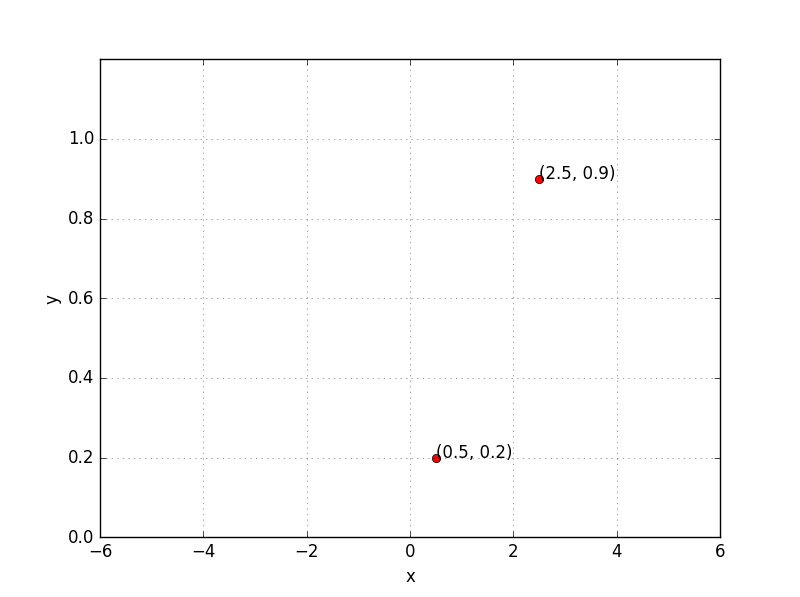
\includegraphics[scale=0.3]{images/module4/2sample_points.png}
				\end{center}
			\end{figure}
		\end{overlayarea}

		\column{0.5\textwidth}<2->
		\begin{overlayarea}{\textwidth}{\textheight}
			\begin{align*}
				\onslide<2->{\intertext{Let's assume there is only 1 point to fit $(x, y)$}}
				\onslide<3->{\mathscr{L}(w,b)                                       & = \frac{1}{2} * (f(x) - y)^2 \\}
				\onslide<4->{\nabla w = \frac{\partial\mathscr{L}(w,b)}{\partial w} & = \frac{\partial}{\partial w} [\frac{1}{2} * (f(x) - y)^2] \\}
			\end{align*}
		\end{overlayarea}
	\end{columns}
\end{frame}

\begin{frame}
	\begin{columns}
		\begin{column}{0.46\textwidth}
			\begin{overlayarea}{\textwidth}{\textheight}
				\begin{align*}
					\onslide<1->\nabla w & = \frac{\partial}{\partial w} [\frac{1}{2} * (f(x) - y)^2]                                                \\
					\onslide<2->{        & = \frac{1}{2} * [2*(f(x) - y) * \frac{\partial}{\partial w}(f(x) - y)] \\}
					\onslide<3->{        & = (f(x) - y) * \frac{\partial}{\partial w}(f(x)) \\}
					\onslide<4->{        & = (f(x) - y) * \frac{\partial}{\partial w}\Big(\frac{1}{1 + e^{-(wx + b)}}\Big) \\}
					\onslide<10->{       & = \color{red}{(f(x) - y) * f(x)*(1- f(x)) *x}}
				\end{align*}
			\end{overlayarea}
		\end{column}
		\vrule{}
		\begin{column}{0.54\textwidth}
			\begin{overlayarea}{\textwidth}{\textheight}
				\begin{align*}
					\onslide<5->{ & \frac{\partial}{\partial w}\Big(\frac{1}{1 + e^{-(wx + b)}}\Big) \\}
					\onslide<6->{ & =\frac{-1}{(1 + e^{-(wx + b)})^2}\frac{\partial}{\partial w}(e^{-(wx + b)})) \\}
					\onslide<7->{ & =\frac{-1}{(1 + e^{-(wx + b)})^2}*(e^{-(wx + b)})\frac{\partial}{\partial w}(-(wx + b))) \\}
					\onslide<8->{ & =\frac{-1}{(1 + e^{-(wx + b)})}*\frac{e^{-(wx + b)}}{(1 + e^{-(wx + b)})} *(-x) \\}
					\onslide<8->{ & =\frac{1}{(1 + e^{-(wx + b)})}*\frac{e^{-(wx + b)}}{(1 + e^{-(wx + b)})} *(x) \\}
					\onslide<9->{ & =f(x)*(1- f(x))*x}
				\end{align*}
			\end{overlayarea}
		\end{column}
	\end{columns}
\end{frame}

\begin{frame}
	\begin{columns}
		\column{0.45\textwidth}
		\begin{overlayarea}{\textwidth}{\textheight}
			\begin{tikzpicture}
	\node [neuron] (neuron0) at (1,6)  {$\sigma$} ;
	\node (input1) at (-1,6)  {$x$};
	\node (input0) at (-1,5)  {$1$};
	\node (output0) at (3,6)  {$y = f(x)$};
	\node (formula) at (0,4) {$f(x)= \frac{1}{1+e^{-(w\cdot x + b)}}$};
	\draw [->] (input0) -- (neuron0);
	\draw [->] (input1) -- (neuron0);
	\draw [->] (neuron0) -- (output0);
\end{tikzpicture}
			\vspace{-0.2in}
			\begin{figure}[!htp]
				\begin{center}
					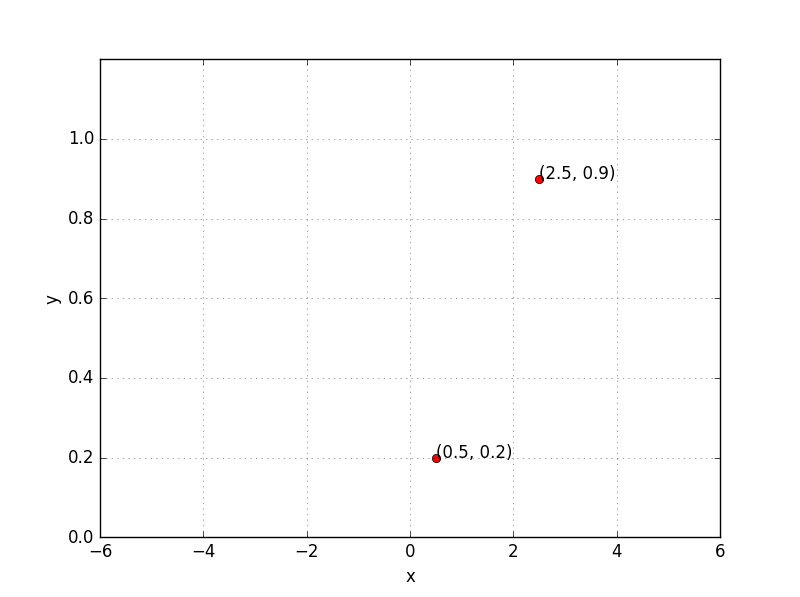
\includegraphics[scale=0.3]{images/module4/2sample_points.png}
				\end{center}
			\end{figure}
		\end{overlayarea}
		\column{0.55\textwidth}
		\begin{overlayarea}{\textwidth}{\textheight}
			\begin{align*}
				\onslide<1->{\intertext{So if there is only 1 point $(x, y)$, we have, }}
				\onslide<2->{\nabla w & = (f(x) - y) * f(x)*(1- f(x)) *x}
				\onslide<3->{\intertext{For two points,}}
				\onslide<4->{\nabla w & = \sum_{i=1}^{2} (f(x_i) - y_i) * f(x_i)*(1- f(x_i)) *x_i} \\
				\onslide<5->{\nabla b & = \sum_{i=1}^{2} (f(x_i) - y_i) * f(x_i)*(1- f(x_i))}
			\end{align*}
		\end{overlayarea}
	\end{columns}
\end{frame}


\begin{frame}
	\begin{columns}
		\column{0.5\textwidth}
		\begin{overlayarea}{\textwidth}{\textheight}
			\vspace{-0.15in}
			\begin{figure}
				\includegraphics<1>[clip,trim=0 650 0 0,scale=0.3]{images/module4/pseudo_code_sgd_crop.png}
				\includegraphics<2>[clip,trim=0 580 0 0,scale=0.3]{images/module4/pseudo_code_sgd_crop.png}
				\includegraphics<3-4>[clip,trim=0 415 0 0,scale=0.3]{images/module4/pseudo_code_sgd_crop.png}
				\includegraphics<5>[clip,trim=0 325 0 0,scale=0.3]{images/module4/pseudo_code_sgd_crop.png}
				\includegraphics<6>[clip,trim=0 235 0 0,scale=0.3]{images/module4/pseudo_code_sgd_crop.png}
				\includegraphics<7>[scale=0.3]{images/module4/pseudo_code_sgd_crop.png}
			\end{figure}
		\end{overlayarea}
		\column{0.5\textwidth}
		\begin{overlayarea}{\textwidth}{\textheight}
			\begin{figure}
				\includegraphics<4->[scale=0.5]{images/module4/error_surface1.png}
			\end{figure}
		\end{overlayarea}
	\end{columns}
\end{frame}


\begin{frame}
	\begin{columns}
		\column{0.5\textwidth}
		\begin{overlayarea}{\textwidth}{\textheight}
			\vspace{-0.15in}
			\begin{figure}
				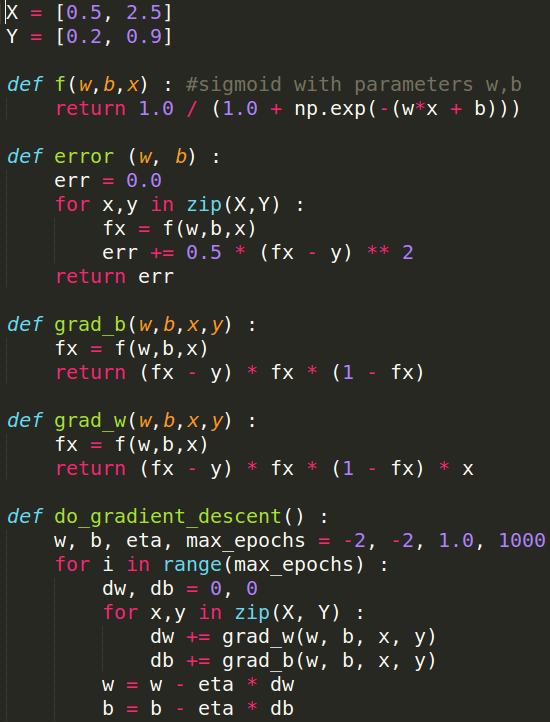
\includegraphics[scale=0.3]{images/module4/pseudo_code_sgd_crop.png}
			\end{figure}
		\end{overlayarea}
		\column{0.5\textwidth}
		\begin{overlayarea}{\textwidth}{\textheight}
			\vspace{-0.15in}
			\begin{figure}
				\foreach \n in {0,...,99} {%
						\includegraphics<\n>[scale=0.5]{images/module4/sgd0/sgd_error\n.png}
					}
			\end{figure}
		\end{overlayarea}
	\end{columns}
\end{frame}

\begin{frame}
	\begin{itemize}\justifying
		\item<1-> Later on in the course we will look at gradient descent in much more detail and discuss its variants
		\item<2-> For the time being it suffices to know that we have an algorithm for learning the parameters of a sigmoid neuron
		\item<3-> So where do we head from here ?
	\end{itemize}
\end{frame}